\vssub
\subsubsection{~Spherical Multiple-Cell (SMC) grid} \label{sub:num_space_SMC}
\opthead{SMC}{\ws (MetOffice)}{J.-G. Li}

\noindent
The Spherical Multiple-Cell (SMC) grid\footnote{~Presently this grid is
activated by a compile switch and can only be used as a stand-alone grid. This
will become a run time option in upcoming model versions.}  \citep{art:Li11}
is an extension of the Cartesian multiple-cell grid \citep{art:Li03} onto the
spherical coordinate system. It is an unstructured grid but retains the
conventional lat-lon grid cells so that all propagation formulations on the
spherical coordinates are still applicable and hence all
the finite difference schemes. The SMC grid relaxes the CFL restriction at
high latitudes in a similar fashion as the reduced grid
\citep{art:RA94}. Polar cells are introduced to remove the polar singularity
of the differential transport equation by switching to an integral
equation. The upstream non-oscillatory 2nd order (UNO) advection schemes
\citep{art:Li08} is implemented on the SMC grid for both spatial and
inter-spectral propagation. This 2nd order scheme can be replaced with a 3rd 
order scheme using the {\F PSMC} namelist logical variable {\code UNO3}.  The UNO3 scheme is similar 
to the UQ scheme but replacing the flux limiters with the UNO 2nd order scheme.  A simple 
rotation scheme is used for wave refraction-induced rotation and the great circle 
turning \citep{art:Li12}.  The refraction scheme is unconditionally stable for 
any time step but the maximum refraction induced rotation angle is limited by 
the maximum possible refraction angle towards the local gradient direction.  
Diffusion term similar to the \cite{art:BH87} for alleviation of the garden 
sprinkler effect is used but the diffusion coefficient is simplified to a single 
homogeneous parameter ($D_{nn}$ as in Eq.~(\ref{eq:Dnn_d})).  An additional 
1-2-1 weighted averaging scheme is also available by the {\F PSMC} namelist logic 
variable {\code AVERG}.  Reduction of computing time with this SMC grid is significant 
in comparison with the conventional grid, thanks to the relaxed time step 
restriction at high latitudes and removal of land points from the model.  
A remedy for the invalided scalar assumption at high latitude is provided to 
extend the global wave model into the entire Arctic Ocean \citep{art:Li16}.  This 
Arctic part can be activated by adding the ARC switch along side the SMC switch.

The SMC grid can be used for replacing the regular lat-lon grid so that the
model domain can be extended to high latitudes or even the North Pole without
reducing the time step. This application requires few changes to the
regular grid model except for preparing a few extra input files, including the
cell array and face array files. The cell array can be generated with the
existing regular grid bathymetry by using the sea points only and merging
cells in the longitudinal directions at a few latitude steps \citep{art:Li11}.

Another important use of the SMC grid is for multi-resolution grids.
The base level SMC grid cell can be refined into 4 quarterly cells
by halving both the longitude and latitude grid lengths. Any cell
on this refined level can be further divided into another 4 quarterly
cells. This refinement can go on as required, resulting in multi-resolution
grids in a few refined levels. For consistency, the single resolution
SMC grid is considered to have only one level.  The normal regular grid input 
files, such as the water depth, land-sea masks, and sub-grid obstruction,
are no longer required, replaced with sea-point only cell and face arrays
and a sub-grid obstruction file.  The water depth is stored in the cell array 
in the last (5-th) column as an integer in meter.  The masks will be defined  
inside ww3\_grid with the sea-point cell array.

Wind and ocean current (if any) forcing can be applied using a regular grid at the base 
resolution as default input forcing for any SMC grid (single or multi-level). 
It will be interpolated on to the refined levels (if any) inside the model.
One option of sea-point only wind and current input for SMC grid can be 
switched on by the {\code SEAWND} logical variable in the {\F PSMC} namelist.  
This sea-point only option not only removes the need to interpolate the wind 
(and current, if any) inside the model but also allows different resolution wind 
(and current) forcings to be mixed up and interpolated to multi-resolution cells 
directly, making it a truly multi-resolution model. 

\begin{figure}
\centerline{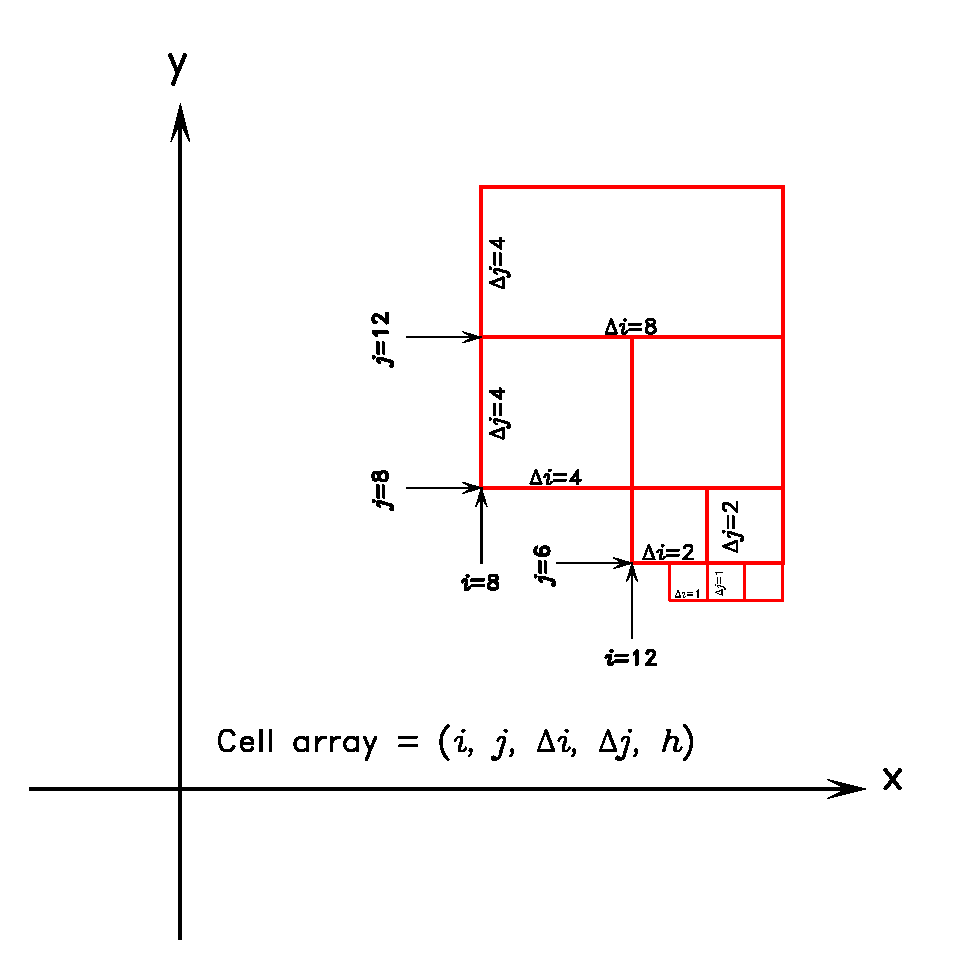
\epsfig{file=./num/smcelary.eps,angle=0,width=3.in}}
\caption{Illustration of cell arrays used in the SMC grid.}
\label{fig:SMCells} \botline
\end{figure}

One important feature of the SMC grid is that it is an unstructured grid, that
is, the cells are not required to be listed side by side as in their physical
position. For the convenience of multi-resolution SMC grid, the cells are
sorted by their sizes so that cells on one given level are grouped together in
one sub-loop for a shared sub-time-step.  The base level time step is halved
as the grid length for the refined level sub-step. This effectively avoids the
model to be slowed down by the refined cells due to their CFL restrictions. 
Neighboring cells information for propagation schemes are provided with cell 
face arrays, which are pre-calculated for the given cell array list. So there 
is no need to expand the sea point only SMC grid cells onto a full grid for 
propagation. Fig.~\ref{fig:SMCells} illustrates how SMC cell arrays are 
defined and Fig.~\ref{fig:SMC_Arctic} shows the Arctic region in a 6-12-25 km 
three level SMC grid. The golden and red circles mark the global and Arctic 
parts in the SMC6-25 grid. The Arctic part within the golden circle requires a 
fixed reference direction to define its wave directional bins. The global part 
(up to the golden circle) can be run independently without the Arctic part. 
The 4 rows from the red to the golden circles are duplicated in the Arctic part 
as boundary cells if the Arctic part is activated with the ARC option.  
Separate cell and face arrays are used for the Arctic part and they are merged 
into the global ones within the wave model for propagation.

\begin{figure}
\centerline{\epsfig{file=./num/JCP_Fig2_GArc.eps,angle=0,width=4.in}}
\caption{The Arctic region in a 6-12-25km multi-resolution SMC grid.}
\label{fig:SMC_Arctic} 
\botline
\end{figure}

Some IDL and F90 programs have been developed for generation of SMC grid cell
and face arrays and visualization of the grid mesh and wave fields but they
have not been formally included in the WW3 package yet. An IDL program 
(Glob50SMCels.pro) is provided in smc\_docs/SMCG\_TKs/ to generate a global 50km 
SMC grid using a 50km regular grid bathymetry ASCII input file (G50kmBathy.dat). 
Face array generation is done with two F90 programs, one for the global part 
(G50SGlSide.f90) and one for the Arctic part (G50SAcSide.f90).  Due to the special 
treatment of the polar cell \citep{art:Li12}, face arrays for the Arctic polar cell 
requires a different approach than other cells. The cell array file has to be 
sorted with a simple Linux script (countcells) before it is fed into the face array 
generation program.  The face arrays also need to be sorted with a Linux script 
(countijsd) to determine the multi-level sub-loop counts.  An independent spectral 
propagation test (G50SMCSRGD.f90) can be run to test the cell and face arrays and 
its output can be visualized with an IDL script, g50smstrspb.pro, which uses the 
saved projection files from the SMC grid visualization program, g50smcgrids.pro. 
By modifying the projection parameters in g50smcgrids.pro, users can choose a 
projection view point (in lat-lon degree) and save the projection for model 
output visualization.  The sub-grid obstruction file can be generated with the 
idl script Glob50SMCObstr.pro.

Compilation of the SMC grid option is similar to that for the regular
lat-lon grid except for that the SMC switch is substituted for the
PR2 UNO combination switches. Note that the SMC grid is built inside
the regular lat-lon grid type so regular lat-lon grid parameters,
such as NX, NY, SX, SY, X1, and Y1, are still required for SMC grid
in ww3\_grid.inp file at the base resolution level. The regular lat-lon
grid water depth, land-sea masks, and sub-grid obstruction input files
are no longer required and they are replaced with SMC grid sea point only 
files (depth is stored in the cell array and subgrid obstruction in 
G50GObstr.dat).  The depth and land-sea mask input lines in ww3\_grid.in 
are, however, kept for passing parameters, such as the minimum depth.
Due to the merges at high latitudes and refined resolutions if any,
regular grid mapping arrays are modified slightly for consistency
with the SMC grid cells. 
Refer to the regression test \emph{regtests/ww3\_tp2.10}
for an example of a 3-level SMC grid model for the Lake Erie.

Output post processing for SMC grid models has been developed for
ww3\_ounf and ww3\_outf. For ww3\_ounf the user can choose between
retrieving multi-resolution information at native model grid sea-points,
or generating regular grids at any of the resolution levels set in
the model grid definition. The ww3\_outf program processes SMC grid data
as either the fully expanded regular lat-lon grid output at the base
resolution level or as ASCII output at all SMC grid sea-points (type-4).
For regular grid outputs, parameter values are determined
using an area-weighted average of all SMC grid cells overlapping the chosen
output cell boundaries. Sea-point data latitudes and longtitudes 
correspond to the native model grid cell centres. For ww3\_ounf
sea-point outputs, variables describing cell sizes are also provided
in the netCDF file.

Visualization tools for sea-point outputs are not provided with this
code release; however some examples are available from the Met Office
on request. For netCDF sea-point outputs a python based GUI tool has
been developed. Visualization of the all cell ASCII output can be done
with the aid of the input cell array file because the output cell 
sequence is the same as the input cell array. The IDL script 
g50smcswhglb.pro is an example program to plot the global 50km SMC grid
SWH output. It uses the projection files produced by g50smcgrids.pro. 
Users are encouraged to develop their own grid-generating and 
post-processing programs in other languages.

It is recommended to read the smc\_docs/SMC\_Grid\_Guide.pdf or the
conference paper \citep{tol:LiS17} at conference web page: 
http://www.waveworkshop.org/15thWaves/
for more information or to contact \url{Jian-Guo.Li@metoffice.gov.uk} 
for any help about the SMC grid.

